\documentclass[a4paper]{article}

%% Language and font encodings
\usepackage[utf8]{inputenc}
\usepackage[T1]{fontenc}
\usepackage{fontspec}
\usepackage[ngerman]{babel}
% Bibliography for lua:
\usepackage[
backend=biber,
bibencoding=utf8
]{biblatex}
\addbibresource{Bibliothek.bib}

%\usepackage[numbers]{natbib} %definition for citation within the text (alternativ option: "numbers"
%\bibliographystyle{plain}
\usepackage{hyperref}

%% Sets page size and margins
\usepackage[a4paper,top=3cm,bottom=2.5cm,left=3.5cm,right=2.5cm,marginparwidth=1.75cm]{geometry}

%% Useful packages
\usepackage{amsmath}
\usepackage{graphicx}
\usepackage{xcolor}
\usepackage{tikz}
\usepackage{wrapfig}
\usepackage{xspace}

\definecolor{backg}{rgb}{0.85,0.85,0.85}

\usepackage{listings} % code formatting
\lstdefinestyle{my}{
    basicstyle = \small\ttfamily,
    keywordstyle=\ttfamily,
    language=bash,
    % morekeywords={
    % },
    backgroundcolor=\color{backg},
    numbers=left,
    commentstyle=\linespread{1.15}\footnotesize\color{olive},
    frame=tlbr, framesep=0.1cm
    }

\lstset{style=my}

\lstnewenvironment{mplisting}
{\newline\minipage[t]{\linewidth}}
{\endminipage \newline}

\newcommand{\inline}[1]{\colorbox{backg}{\lstinline{#1}}}
\usepackage{dirtree} 
\newcommand{\qq}[1]{\textit{\glqq#1\grqq}\xspace}

\makeatletter
\title{Versionskontrollsystem Git}\let\Title\@title
\author{Till Hanke}          \let\Author\@author
\date{\today}           \let\Date\@date
\makeatother



\begin{document}
\begin{titlepage}
	\centering
	{\scshape\LARGE Martin-Luther-Universität Halle-Wittenberg \par}
	\vspace{1cm}
	{\scshape\Large Bericht\par}
    zum Orientierungspraktikum\\
	\vspace{1.5cm}
	{\huge\bfseries \Title\par}
	\vspace{2cm}
    vorgelegt von\\
	{\scshape\Large \Author\par}
	\vfill
	\begin{flushleft}
    \begin{tabular}{llll}
    \textbf{Halle (Saale), den:} & & \Date &\\
    				& & \\
    \textbf{Betreuer:} & & Prof. Ingrid Mertig &\\
%    \textbf{2. Gutachter:} & & PD Dr. Jürgen Henk &\\
    \end{tabular}
    \end{flushleft}
    % Bottom of the page
\end{titlepage}
\newpage
\tableofcontents
\newpage
\section{Einleitung}
Ein großer Teil der Forschung in der Physik umfasst das Schreibenund Entwickeln umfangreicher Programmcodes. Diese werden meist über Jahre oder gar Jahrzehnte hinweg aufgebaut. Viele Codes werden von gro"sen Gruppen gemeinsam weiter entwickelt. Um Programmcode effizient zu dokumentieren und Änderungen auch Jahre später noch rückverfolgbar zu machen wurden Versionskontrollsysteme entwickelt. Diese Systeme sollen einen Überblick verschaffen über den Verlauf von Änderungen, aber auch die Zuordnung von Änderungen zu Personen ermöglichen. Mittlerweile nutzen fast alle Entwickler Git als Versionskontrolle. Dafür werden zumeist auch öffentliche Server (\url{Gitlab.com} oder \url{Github.com}) genutzt um den gesamten Code der Community zur Verfügung zu stellen\footnote{Der Quelltext dieser Arbeit steht auf Github zur Verfügung unter: {\url{https://github.com/tillhanke/git-basics}}}.

In dieser Arbeit sollen die Grundlagen der Arbeit mit Git erklärt werden. Der Fokus liegt dabei auf dem Arbeiten alleine mit einer dezentralen Sicherung des Codes. Zusätzlich wird am Ende auf die gemeinschaftliche Arbeit mit Git eingegangen.

Alle Instruktionen in dieser Arbeit beziehen sich auf Linux Betriebssysteme. Die meisten der angegebenen Befehle werden auch auf MacOS Systemen funktionieren. Git ist auch für Windows OS verfügbar jedoch wird darauf in dieser Arbeit nicht eingegangen. Auch wird die Installation von Git auf den genutzten Maschinen vorausgesetzt.

\subsection{Versionskontrolle}
Das Ziel einer Versionskontrolle wie Git ist es die Änderungen an einem Projekt zu dokumentieren. In Abb. \ref{fig:vers-kontrol}
ist eine solche Protokollierung visualisiert. Um Änderungen zu verfolgen werden zu jeder Änderungen Kommentare hinzugefügt - sogenannte "Commit-Messages". Diese Kommentare sollen das spätere zurückverfolgen der Änderungen vereinfachen. Um Speicherplatz zu sparen sollen in der Versionskontrolle möglichst nicht alle Dateien zu jedem Zeitpunkt gespeichert werden. Es wird somit nur einmal (zum Zeitpunkt der Erstellung) die komplette Datei gesichert. Danach werden von jeder Datei nur Informationen über die Änderungen abgespeichert.
\begin{figure}[!h]
    \centering
    \includegraphics[width=0.9\textwidth]{Bilder/Versioncontrol.png}
    \caption{Beispiel Versionskontrolle von drei Änderungen an zwei Dateien desselben Projekts. Eingezeichnet sind zwei protokollierte Stadien des Projekts. Zu jeder Änderung ist ein Änderungskommentar angegeben.}
    \label{fig:vers-kontrol}
\end{figure}

\newpage
\section{Initialisierung eines lokalen .git}
Git muss in dem Hauptordner eines Projektes initialisiert werden. Das bedeutet, dass alle Projekt-Dateien in Unterordnern zu finden sein müssen (eine Exemplarische Ordnerstruktur ist in \ref{fig:dir_struc} dargestellt). Bei der Initialisierung von Git wird im Hauptordner zusätzlich ein neuer Unterordner  \inline{.git/} angelegt. In diesem Ordner wird Git alle Versionsinformationen und die Historie abspeichern. Durch Löschen des Ordners kann man Git von dem Projekt trennen.
\begin{figure}[!h]
    \dirtree{%
    .1 Git-Basics.
    .2 .git.
    .3 \ldots \hspace{2ex}\begin{minipage}[t]{8cm}In diesem Ordner werden die Informationen über Änderungen abgespeichert\end{minipage}.
    .2 Bilder.
    .3 git\_commit.png.
    .3 Versioncontrol.png.
    .2 main.tex.
    .2 Title.tex.
    .2 initialisierung.tex.
    .2 Einleitung.tex.
    .2 Commit.tex.
    .2 Bibliothek.tex.
    }
    \caption{Exemplarische Ordnerstruktur für ein Projekt mit Git.}
    \label{fig:dir_struc}
\end{figure}

Um in einem Projektordner Git zu initialisieren genügt der Befehl 
\begin{mplisting}
$ git init
\end{mplisting}
Dadurch wird in dem aktuellen Verzeichnis ein \inline{.git} Ordner angelegt.
%
\subsection{Git Config}
Um Änderungen zu protokollieren benötigt Git Informationen über den User. Diese Informationen können System-übergreifend, pro User oder für das jeweilige Projekt hinterlegt werden. Die benötigten Informationen sind Email-Adresse und Benutzername. Definiert werden können die Informationen mithilfe von \inline{git config}. Durch die Angabe einer Option wird definiert ob diese Information für das System (\inline{--system}), den User (\inline{--global}) oder das Projekt (\inline{--local}) abgespeichert werden sollen.
\begin{lstlisting}[breaklines=true]
$ git config --global user.name "Max Mustermann"
$ git config --global user.email "max@mustermann.de"
$ git config --global core.editor vim  # Dieser Editor wird von git genutzt um Eingaben des Users ab zu fragen.
\end{lstlisting}
Nach der Initialisierung kann der Status des Git mit \inline{git status} abgefragt werden.
\begin{mplisting}
$ ls -a
.   Bibliothek.bib  Commit.tex      .git                 main.tex
..  Bilder          Einleitung.tex  initialisierung.tex  Title.tex
$ git status
On branch master

No commits yet

Untracked files:
  (use "git add <file>..." to include in what will be committed)
	Bibliothek.bib
	Bilder/
	Commit.tex
	Einleitung.tex
	Title.tex
	initialisierung.tex
	main.tex

nothing added to commit but untracked files present (use "git add" to track)

\end{mplisting}
Durch diese Initialisierung wurde ein leeres Git-Repository angelegt. Jedoch hat das Repository noch keine Dateien, deren Verlauf protokolliert werden soll. Um Dateien der Versionskontrolle hinzu zu fügen müssen diese zum Repository hinzugefügt werden. Das geschieht über den \inline{git add} Befehl.
\begin{mplisting}
$ git add main.tex
$ git status
On branch master

No commits yet

Changes to be committed:
  (use "git rm --cached <file>..." to unstage)
	new file:   main.tex

Untracked files:
  (use "git add <file>..." to include in what will be committed)
	Bibliothek.bib
	Bilder/
	Commit.tex
	Einleitung.tex
	Title.tex
	initialisierung.tex
\end{mplisting}
Um alle Dateien des Ordners, und der Unterordner dem Repository hinzu zu fügen kann man den Hauptordner hinzufügen.
\begin{mplisting}
$ git add .
$ git status
On branch master

No commits yet

Changes to be committed:
  (use "git rm --cached <file>..." to unstage)
	new file:   Bibliothek.bib
	new file:   Bilder/Versioncontrol.png
	new file:   Bilder/git_commit.png
	new file:   Commit.tex
	new file:   Einleitung.tex
	new file:   Title.tex
	new file:   initialisierung.tex
	new file:   main.tex

\end{mplisting}
Damit wurden alle Dateien der Versionskontrolle hinzugefügt. In Git nennt sich der Zustand, in dem die Dateien sich hier befinden \qq{Staging}. Noch hat Git die Änderungen nicht protokolliert, sondern nur die Dateien markiert um sie bei dem nächsten Commit zu protokollieren. Die vier Stadien, in denen sich eine Datei in Git befinden kann sind in Abb. \ref{fig:lifecycle} dargestellt. Der \inline{git add} Befehl hat die Dateien von \qq{untracked} auf \qq{staged} gesetzt.
\begin{figure}[!h]
    \centering
    \includegraphics[width=\textwidth]{Bilder/lifecycle_de.png}
    \caption{Die 4 Zustände, in denen eine Datei sich im Git befinden kann. Die Pfeile geben an, wie die Dateien zwischen den Stadien wechseln. Das Bild wurde aus \cite{ProGit} entnommen und leicht verändert.}
    \label{fig:lifecycle}
\end{figure}

%
\newpage
\section{Erster Commit}
\begin{lstlisting}
$ git add README.md
$ git status
On branch master

No commits yet

Changes to be committed:
  (use "git rm --cached <file>..." to unstage)
        new file:   README.md
\end{lstlisting}
An dieser Stelle wurde die Datei
\inline{README.md} dem nächsten Commit hinzugefügt. Um den Aktuellen Status zu protokollieren muss der Befehl \inline{git commit} genutzt werden. Dabei werden alle Änderungen Protokolliert.
Git speichert intern die Version der Datei ab und verweißt in jedem folge Commit darauf. Wenn die Datei nicht verändert wird wird somit nicht mehr Speicherplatz verwendet, egal in wie vielen Commits die Datei vorkommt.
Ein commit wird immer mit einer Commit-Message begleitet. Wenn der Befehl \inline{git commit} ohne Optionen ausgeführt wird öffnet sich daher automatisch der standard editor (der über \inline{git config --local core.editor} definiert wurde). In diesem Befindet sich eine auskommentierte Übersicht des Commits. Darunter muss eine Commit-Message eingefügt werden.
\begin{figure}[!h]
        \centering
        \includegraphics[width=0.5\textwidth]{Bilder/git_commit.png}
        \caption{Eine Commitbaum-Darstellung von XKCD \cite{Munroe}. Die Commit-Messages starten oben mit den ersten Commits sehr vorbildlich. Nach einigen Commits ist zu sehen, dass die Messages keine informationen über den Commit Inhalt mehr haben. Dies ist ein häufiges Problem, wenn zu selten Committed wird kann es schnell passieren, dass nicht mehr klar ist, was sich seit dem letzten Commit alles geändert hat. Dadurch werden Commit-Messages schnell schwer zu schreiben und vernachlässigt.}
        \label{fig:commit-XKCD}
\end{figure}

Commit-Messages sollten 
%
\newpage
\section{Branches}\label{sec:branch}
Während der Entwicklung eines Programms ist es meist nützlich mehrere Versionen parallel zu verwalten. Das kann heißen, dass es eine \qq{release} Version und eine \qq{developement} Version gibt. Oder, dass man die letzte funktionierende Variante des Programms erhalten will während man neue Funktionen versucht zu implementieren.

Das parallele nutzen von Entwicklungssträngen ermöglichen Branches in Git.
\subsection{Branch erstellen}
Um einen Branch zu erstellen ruft man \inline{git branch} mit einem Namen für den Branch auf. Dann kann mit \inline{git checkout} zu dem Branch gewechselt werden. Der Log zeigt die Stadien der Branches ebenfalls an.
\begin{lstlisting}
$ git branch section4
$ git checkout section4
$ git log --pretty=format:"%h %s %d"
04965ab add: sentence at end of Commit  (HEAD -> section4, master)
906a721 add: label for future sections 
03a1fee add: Subsection about reverting commits 
bf11cfe add: files to ignore from macOS 
\end{lstlisting}
Hier kann man sehen, dass sowohl master, als auch section4 auf denselben Commit zeigen (\inline{04965ab}). Jeder neue Commit jedoch wird nur von section4 erfasst, nicht von dem master Branch.

\begin{figure}[!ht]
	\centering
	\includegraphics[width=0.4\textwidth]{Bilder/branching.png}
	\caption{Beispielhafter Branch-tree aus diesem Projekt. Graue Kästen stellen einzelne Commits dar, orangene Branches und der gelbe Kasten ist der aktuelle HEAD. Die Pfeile zeigen auf die Verlinkung.}
	\label{fig:branch_1}
\end{figure}
Abb. \ref{fig:branch_1} zeigt den Branch-tree des Gits nach dem ersten Commit in section4. \inline{HEAD} zeigt immer auf den aktuellen Zustand des lokalen Ordners. In diesem Fall auf den Branch section4. Die Branches selber zeigen auf den Commit, den sie gerade darstellen. Um den \inline{HEAD} zu wechseln muss nur \inline{git checkout [BRANCH]} mit dem entsprechenden Branch aufgerufen werden.
\begin{figure}[!ht]
	\centering
	\includegraphics[width=0.4\textwidth]{Bilder/branching_2.png}
	\caption{Branch-tree nachdem mehrere Commits zu den Branches gemacht wurden.}
	\label{fig:branch_2}
\end{figure}

\subsection{Merging}
Das Zusammenführen zweier Branches wird Merging genannt. Dabei ist es das Ziel, alle Änderungen der beiden Branches in einem Branch zu vereinen. Wichtig ist, dass immer der Branch ausgewählt (HEAD zeigt darauf) sein sollte, in dem man die Änderungen vereinen will. Will man also in master die Änderungen von section4 einbinden geht das folgendermaßen:
\begin{lstlisting}
	$ git checkout master
	$ git merge section4
	Merge made by the 'recursive' strategy.
	Bilder/branching.png   | Bin 0 -> 25763 bytes
	Bilder/branching.svg   | 648 ++++++++++++++++++++++++++++++++++++++++++++++++++++++++++++++++++++++++++
	Bilder/branching_2.png | Bin 0 -> 41671 bytes
	branches.tex           |  36 +++++
	main.tex               |   3 +-
	5 files changed, 686 insertions(+), 1 deletion(-)
	create mode 100644 Bilder/branching.png
	create mode 100644 Bilder/branching.svg
	create mode 100644 Bilder/branching_2.png
	create mode 100644 branches.tex
\end{lstlisting}
Merging ist ein einzelner Commit. Dieser Commit zeigt auf die beiden Commits, auf welche die einzelnen Branches vorher gezeigt haben (siehe Abb. \ref{fig:merge}). Nachdem ein Branch gemerged wurde kann er gelöscht werden.
\begin{figure}[!ht]
	\centering
	\includegraphics[width=0.6\textwidth]{Bilder/branching_3.png}
	\caption{Branch-tree nach dem Merging. Der Merge wird als eigener Commit oberhalb der beiden child-Commits angezeigt. Der master Branch und HEAD zeigen beide auf den Merge-Commit. Der section4 Branch existiert weiterhin, zeigt jedoch auf den alten Commit.}
	\label{fig:merge}
\end{figure}
% - mergeconflicts not yet included
%
\newpage
\section{Remotes}
Ein Git kann nicht nur lokal geführt werden. Wirklich effektiv werden Gits wenn man sie mit einem remote-Server verbindet und somit mit anderen Personen teilen kann. Der Server kann auf verschiedenste Arten erreichbar sein. Die häufigsten Methoden einen remote-Server an zu sprechen sind jedoch http(s) und ssh. 
\subsection{Github}
Es gibt online verschiedene Anbieter für Git-Server. \url{Github.com} ist einer der wohl bekanntesten. Um ein Projekt bei Github zu veröffentlichen (oder privat dort zu sichern) muss lediglich ein Benutzeraccount angelegt werden.

In diesem Beispiel wird gezeigt, wie man ein lokales Git per SSH auf Github synchronisieren (\qq{pushen}) kann und Github somit als Remote ein zu richten. Um ssh mit Github zu verwenden muss ein SSH-Schlüssel auf dem lokalen PC erstellt werden, und der öffentliche Schlüssel bei Github hinterlegt werden. Ein SSH-Schlüssel kann mit \inline{ssh-keygen} erzeugt werden. Als Standard wird dadurch ein RSA Schlüssel-Paar erzeugt und im \inline{/home/user/.ssh/} Ordner hinterlegt.
Es entstehen in diesem Ordner \inline{id_rsa} und \inline{id_rsa.pub} die Datei, die mit .pub endet enthält den öffentlichen Schlüssel, der weitergegeben werden kann. Die andere Datei sollte niemals weitergegeben werden. Sie enthält den privaten Schlüssel, mit dem man sich dann authentifizieren kann.
\begin{mplisting}
$ ssh-keygen  # erzeugen eines Schlüsselpaares
$ cat ~/.ssh/id_rsa.pub  # anzeigen des öffentlichen Schlüssels
ssh-rsa
AAAAB3NzaC1yc2EAAAADAQABAAABgQDMuksDJfybOInEWtN+tSxLmjT/wG5q6ZY4aZFRB
lhoho865XwJZZm1DAdL0Ec9Lt1DfHfAhX9QOTlJW1qXX6dn1dtD5ih6n41tdxpxxJ/P2a
6YHGGKYQ0p7qSqzS5ydu+GST73lWxK8eDrU8Tm+lDRpyGu4GRqph5gemFyzW11AD2OknW
cm+Zp9ghHWUZuGGH8KqYWAHjkMDuZZMchC4f7IhrVZwhiiWFMyS7BEaIb8FrKtpTnjeoH
4qkaHNr8umFxatZRLYqHMrx/JA0/4JwLFNOtZTVTl220Nst5+cCx54ZhDHi1AeROMZ5xw
BPiYHi3eBsEfHZBt6euJNWcdVoq6bZK+ImXA1IszqevJNu571g9sBHjOtkgrXVoYVicnC
wGYI2Fnd4VRjPV+4xSLnizqr0fMvXlGdTvlyXML4gA+eyYwBF83xQ35F2e8FA+dGCzyGL
7A/zd1yDh1jVgsiQMVwuA3xVEGWnVzo6kXk/qCuMaIivLi3R9vuokdwL+iak= till@phys-87
\end{mplisting}
Dieser öffentliche Schlüssel kann nun bei Github unter \inline{settings -> SSH and GPG keys -> New SSH key} eingegeben werden. Damit kann man von dem Rechner aus, auf dem der Schlüssel hinterlegt ist, auf jedes Github Repository des Benutzeraccounts zugreifen.

\subsection{Remote hinzufügen}
Mit \inline{git remote} kann man alle verknüpften Remotes auflisten lassen (wenn keine Remotes eingerichtet sind sollte das also keine Ausgabe erzeugen). Um ein Github Repository als Remote mit dem lokalen Repository zu verknüpfen muss zuerst ein Github Repository online erstellt werden. Diesem neuen Repository wird ein Name gegeben, nach der Erstellung kann das lokale Repository mit Github verbunden werden.
\begin{mplisting}
$ git remote add github git@github.com:[Benutzername]/[Github Repo Name].git
$ git remote
\end{mplisting} 
Dabei muss der remote Verknüpfung ein Name gegeben werden (hier \inline{github}) und der Link zu dem remote Repository angegeben werden (bestehend aus dem Benutzername und dem Namen des Github Repository). \inline{git remote} sollte daraufhin den Namen des gerade hinzugefügten remotes auflisten (\inline{github}). Damit ist das lokale Repository jedoch noch nicht auf Github zu sehen. Um den aktuellen Stand des lokalen Repositories zu Github zu pushen muss \inline{git push} genutzt werden.
\begin{mplisting}
$ git push github master
\end{mplisting}
\inline{git push} benötigt mindestens zwei Argumente. Das erste Argument gibt den remote an zu dem gepushed werden soll (es können mit einem lokalen Repository mehrere remotes verbunden werden) das zweite Argument gibt den Branch an, der gepushed werden soll. Durch diesen Befehl wird der lokale Branch mit dem remote Branch gemerged. Falls das remote Repository diesen Branch noch nicht hat wird dieser erzeugt.
% - ssh custom server remote
% - gitlab/github with https
%
\newpage
\nocite{*}

\printbibliography

\end{document}